\section {Problem Introduction}
In the traditional Internet architecture, a single server (or server pool in one data center) handles multiple incoming client requests.  
The bottleneck in such systems under high load can be lack of bandwidth to and from the server \cite{coopnet}, because bandwidth is split $N$ 
ways among the requesting clients (see Fig. \ref{fig:traditional_http}).  When an increasing number of clients request a web page, that page 
therefore loads more and more slowly for users.  This problem occurs anytime the ratio of bandwidth to clients is low.  For example, when a server 
is poorly provision, a server experiences spikes in load, or a small number of incoming clients download very large files.  An example of this problem 
is the ``slashdot" effect, in which a sudden flash crowd of clients suddenly requests certain (news-worthy) pages, overwhelming unexpectant servers
.  These situations cause web servers to become overwhelmed and even crash.

\section {Related work}
This problem is commonly combated by distributing the requests among a set of servers that mirror the content of the original server (Fig. \ref{fig:server_only}).  
A company establishes mirrors by locating a set of servers in many different places on the Internet, then automatically redirecting clients to these servers, thus 
distributing the load to provide better performance.  An example of this is the large commercial CDN run by Akamai \cite{akamai}, which performs distributed
downloads for its clients (for example Apple uses it to distribute their iTunes\texttrademark  program).  This solution however requires a dedicated pool of 
servers to provide the extra bandwidth.  Not all sites can afford a CDN, and the mirrors require cooperation, configuration, and maintenance, hence their expensive.

As a cheaper alternative, many web sites are beginning to use \emph{peer-to-peer content distribution}, or \emph{swarming}, with BitTorrent.  In BitTorrent, clients 
download only parts of a file from a central server, and download the rest of it from their peers in the system.  While a client participates, it is both downloading 
the parts (blocks) it needs and uploading the blocks it has to other peers (see Fig. \ref{fig:normal_swarm}).  Peer-to-peer content distribution enables a 
web server to serve a large file to a large numbers of users with good speeds \cite{zappala}. Swarming protocols have been shown to actually decrease total download 
time per peer as the number of peers increases, which is the opposite of the traditional client-server paradigm \cite{slurpie}. 

\begin{figure}
\begin{center}
   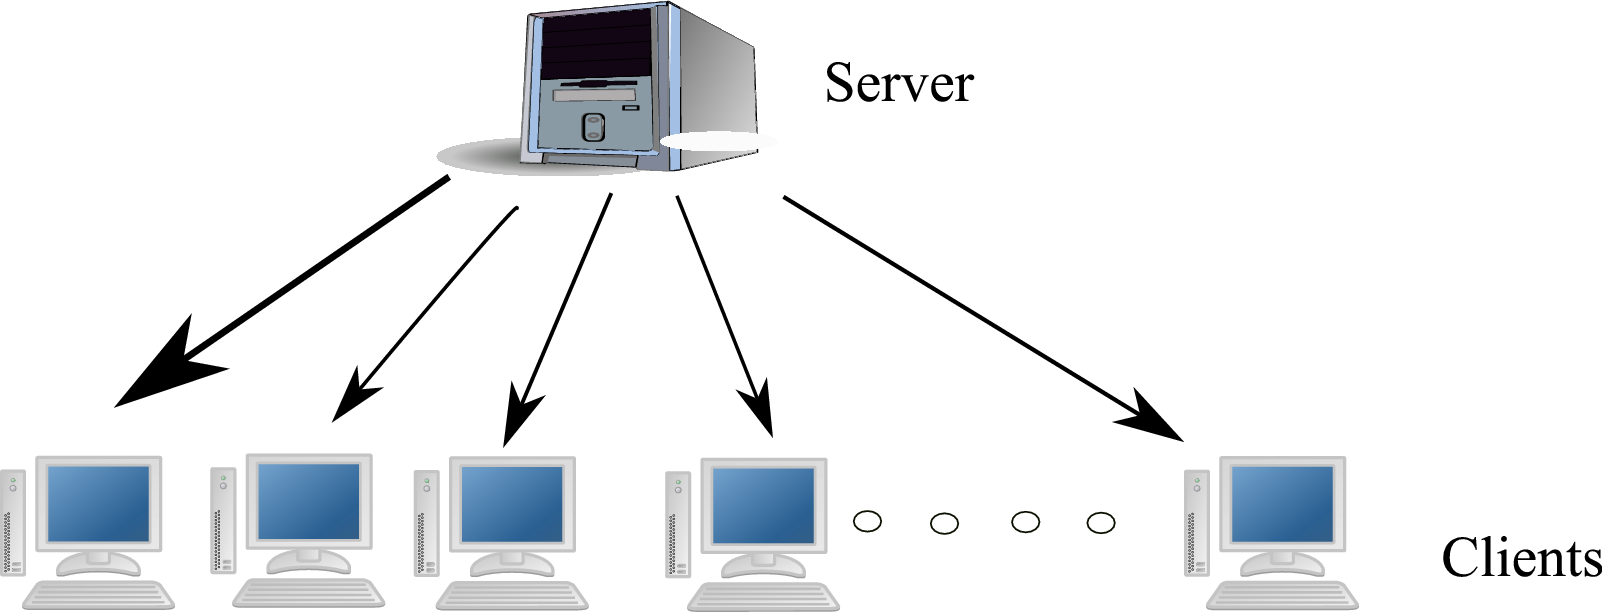
\includegraphics[width=11cm]{description_pics/traditional_http.png}
    \caption{Traditional HTTP download}
 \label{fig:traditional_http}
 \end{center}
\end{figure}
\begin{figure}
    \centering
  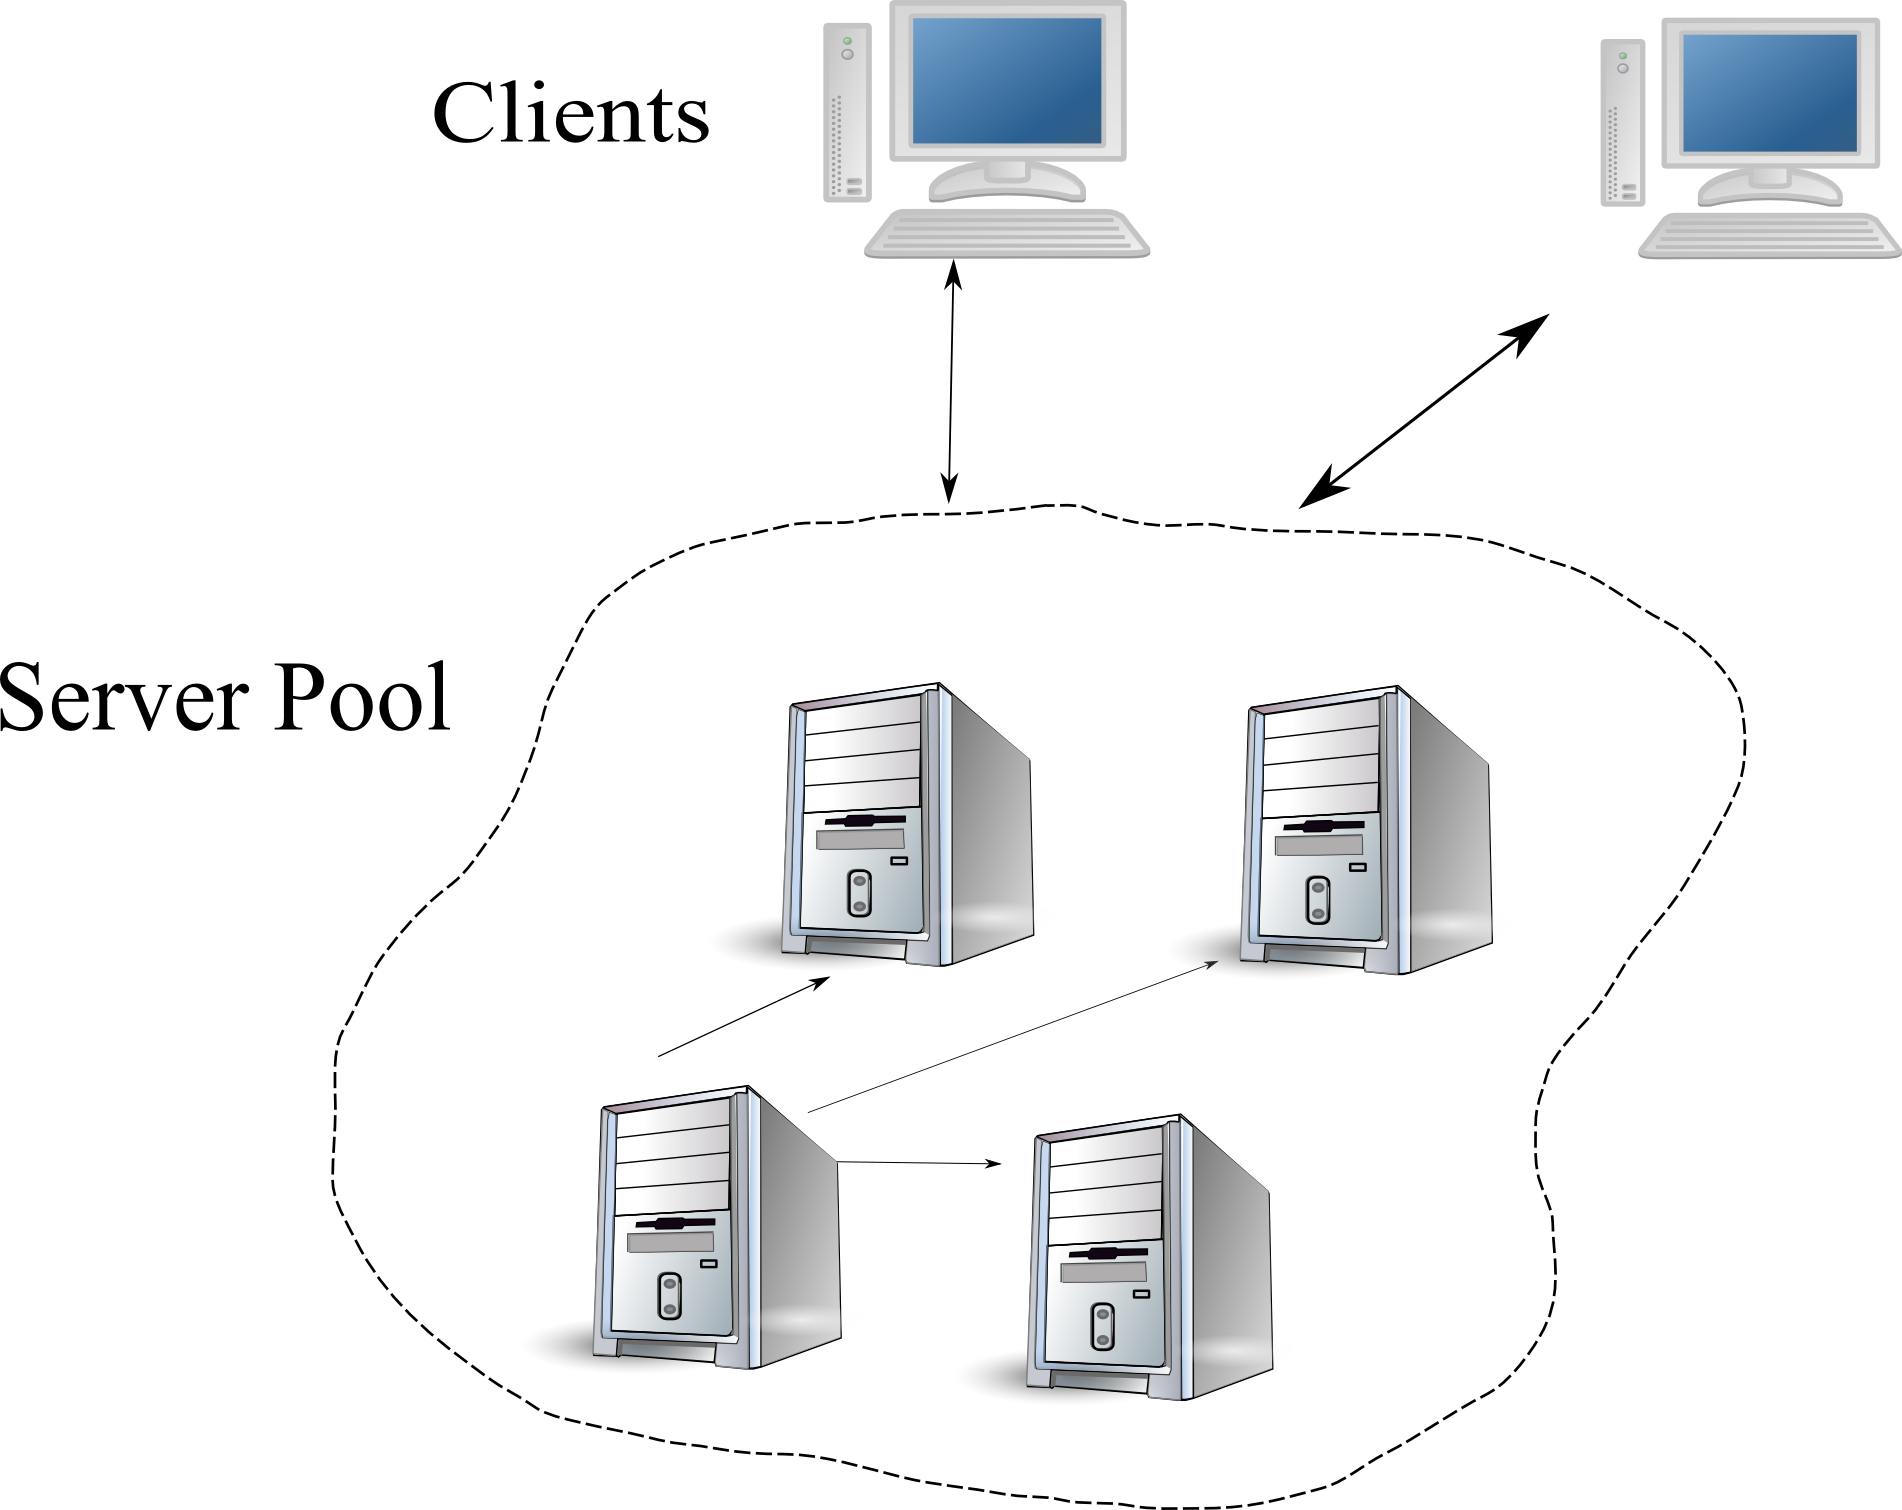
\includegraphics[width=8cm]{description_pics/server_side_only.png}
  \caption{Server CDN example}
  \label{fig:server_only}
\end{figure}   
\begin{figure}
 \centering
 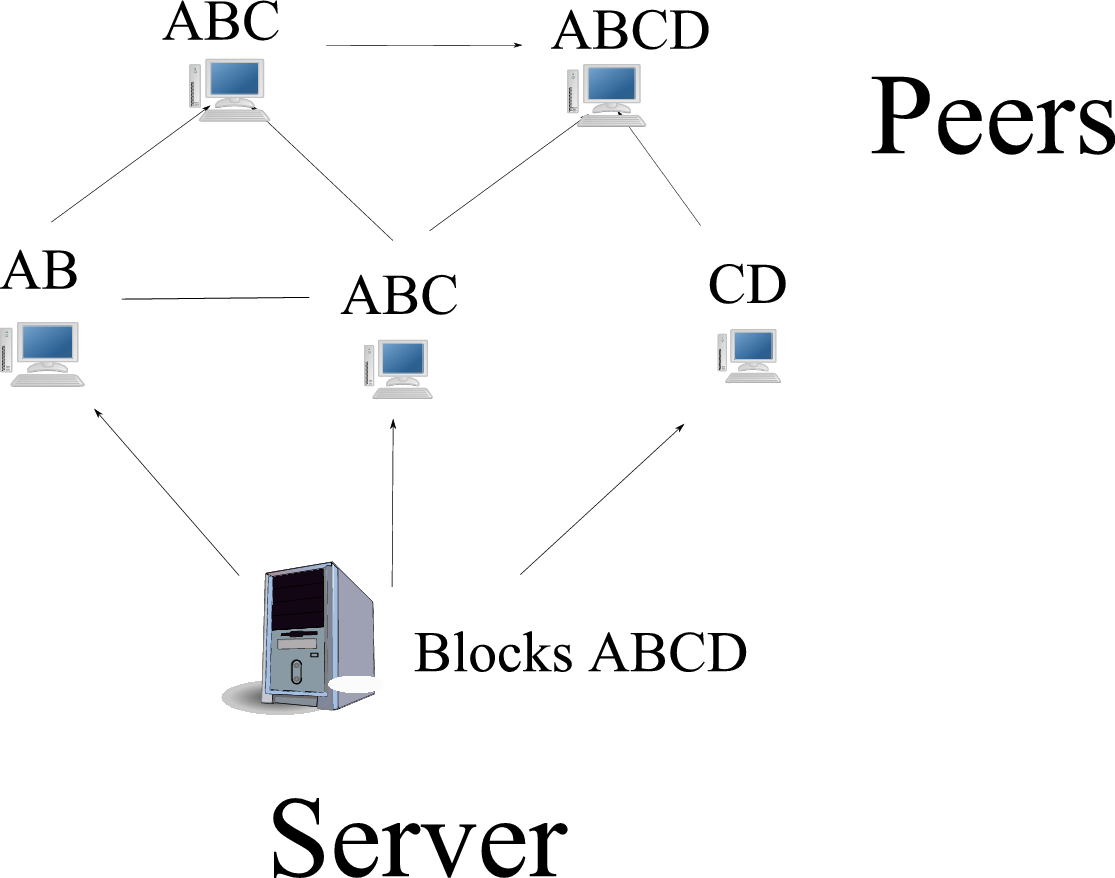
\includegraphics[width=4.5cm]{description_pics/normal_swarm.png}
 \caption{Swarming example.  Arrows represent block exchanges.}
 \label{fig:normal_swarm}
\end{figure}

BitTorrent, however, currently requires setup for both servers and users, and isn't well-integrated into normal HTTP downloads.  BitTorrent peers first locate a 
file with a ``.torrent'' extension from an out of band source such as a web server.  This file lists a target file's size, MD5 hashes of the blocks of the file, and 
the IP address of a tracker for that file.  This tracker is a dedicated machine which helps connect the peers to each another.  Peers contact the tracker to receive 
a list of peers who are currently downloading the file.  They then establish connections and begin sharing and receiving blocks with their neighbors.

%->final ?:BitTorrent, for the download of the last block of a file, uses a kind of 'many peers downloading the same blocks.  It requests the last block simultaneously from many peers, so that if one peer is transmitting it very slowly, they will be quickly passed by one of the faster seeds, and thus download it quickly.

BitTorrent is not commonly used for serving all the files of a web site.  It is used mostly for large files, and requires configuration on both the server and client sides.  
Every file shared has a .torrent file must be created, and a tracker established for that file\footnote{There have been some proposals of integrating BitTorrent with Apache
 \cite{webtorrent}, which show that even if a few clients contribute it helps with speedup, however this is mostly proposed as a server and client-side solution.  
 There are applets that will download BitTorrent files, and FireFox plugins to make downloading more seamless, but it still has a high barrier to entry for most users, 
 and servers must understand the protocol.}.  This type of configuration is difficult for an entire web site, and typically requires users to switch browsers in order to complete the download.  
 This somewhat manual process is non user-friendly for small files, for example those of a web page.  BitTorrent also employys incentives to share blocks of files, which can cause longer boot-strapping 
 time for new peers, which is poorly suited to small file downloads.  Recent improvements to BitTorrent include a ``trackerless'' option, which means peer lookup is 
 shared amongst the peers themselves, but access to the original .torrent files is still centralized (.torrent files must still be created).  This design requires 
 that all web servers and clients know and use a peer-to-peer protocol, causing a barrier to entry (for example, download sites offer links to BitTorrent downloads 
 which are ignored).

\section {Thesis Statement}\label{section:thesis}
Our hypothesis is that a system of cooperating web clients can reduce load on an origin web server by automatically switching from client-server file transfer to
 peer-to-peer content delivery.  This system can provide fast download times for objects of many sizes, especially small files.  It should be equivalent in speed 
 to BitTorrent for larger files, without requiring any manual configuration or participation from web servers.

\section{Related Work}\label{section:related_work}
Much work has been done to distribute file downloads.  Solutions fall into three basic categories: client-side protocols, client and server-side protocols, 
and server-side protocols.  Each category has certain trade-offs and advantages.

\subsection{Client-Side Only Protocols}
Protocols that use only client-side protocols are popular in the literature.  Client-side protocols involve peers self-organizing to share content.  
These solutions require no change in the server software, allowing them to be implemented without requiring servers to be aware of the changes.  However, 
this requires that clients must self-organize without the help of the centralized server.  Our protocol follows this pattern.

Shared web caches are another example of a client-side only protocol.  They allow peers to download files from some well known cache--typically a specific 
set of computers, such as those run by PlanetLab.  Coral \cite{coral} and CoDeen \cite{codeen} are examples of such caches.  Shared caches can be effective, but
cache systems like coral and CoDeen typically require a dedicated set of proxies.  They are constrained to the number of participating proxies, and they 
require an infrastructure of hosts who are willing to be dedicated to serving bandwidth, which is rare and expensive.  
In extreme cases (load surpassing the bandwidth of the combined sum of proxies), these systems still become overburdened, in the case of Coral, they are
limited to 4.5GB transfer per day per host.  Because of this, if Coral receives a request for a file too many times, it begins redirecting peers back to 
the origin server, thus becoming less effective.  Coral is also limited in the size of files it can cache by the size of disks on PlanetLab proxies.  
With our system this should not be a problem, as more peers means resources are available to upload.  These systems also lack an algorithm for transition 
to peer-to-peer download, and swarming.  CoDeen also adds an extra hop in network latency per request, even if a request from the origin server would have 
been the fastest way to download the file, thus causing slowdown in some cases.

Squirrel \cite{squirrel} is another shared web cache.  Squirrel clients join a local DHT and cache any files that 
map to their location in the DHT.  The DHT is used to locate the peer owner who then serves as proxy for that file.  The advantage of this is it doesn't 
require dedicated infrastructure.  The disadvantage is it does not offer an algorithm for transparent transition to p2p download, nor does it allow for 
partial file downloads (swarming).

%The effect of  flash crowds can also be alleviated by searching among a random subset of Internet peers for desired files.  PROOFS \cite{proofs} (P2P Randomized Overlays to Obviate Flash-crowd Symptoms) uses flooded search to allow peers to locate 'popular' or 'flash crowded' files from other peers who have previously downloaded the same.  The creators conjecture that files that are the subjects of a flash crowd are likely to be locatable among random sets of peers, since they are popular, hence their use of a random flood search.  The benefit of this system is that nodes need not maintain a structured search system (such as a DHT). However, not having a DHT for lookup makes searches more random and slightly less accurate, with potentially higher overhead.  PROOFS also does not include parallel downloads nor offer a protocol for automatic transition to a peer-to-peer solution.

Overall, client-side solutions alleviate flash-crowds. There are few that provide automatic transition to peer-to-peer (swarming-style) download.

\subsection{Server-side and Client-side Cooperative Protocols}

The most popular type of load alleviation currently is a server and client-side cooperative protocol, BitTorrent,  developed in 2001 by Bram Cohen \cite{cohen}.
%Many file distribution protocols include some cooperation and previous knowledge between the server and client.  In these protocols clients typically access blocks of a file from the server and also from peers.  Server-side and client-side cooperative protocols basically fall into two categories: those used for web redirection, and those used to download single objects.  For web redirection, servers typically redirect clients to former clients that have downloaded files previously \cite{pseudoserving, coopnet}.  This allows a server to 'meter' its upload speeds and redirect peers, when appropriate, thus providing a backup strategy for over-loaded servers.  An example of this is the pseudo-server system \cite{pseudoserving}.  This style of protocol typically requires changes to both the server and client software, however, and the server could still become overloaded in extreme cases.
Some other related protocols incorporate web-redirection (i.e. the server redirects peers to recent downloaders \cite{overhaul, webtorrent, onion, zappala, cohen,
slurpie, mutualcast, fastreplica, avalanche, bullet_prime, onion}).  
Swarming provides the benefit of scalable downloads of large files.  
%OnionNetworks, for instance, proposes an extension to HTTP to allow  HTTP response messages to include hashes of files and a list of peers from to which other peers may connect and download in a 
%swarming fashion \cite{onion}.  Unfortunately their proposal has not seen wide-spread adoptance, nor research.  
They are highly effective at serving loads orders of magnitude higher than an ordinary web server \cite{zappala}. 
Current protocols requires extra setup for both client and server, however.
The biggest disadvantage of this style architecture is that it requires adoptance on both the server and client sides.

The Shark \cite{shark} filesystem allows clients to download blocks of files from nearby neighbors who have blocks already on their local machines.  
Shark is similar to our proposed system, except applied to files in a file system, not web objects.  
It requires a custom DHT for peer localization and proximity estimation, and a central server for hash values of files.  
It also lacks HTTP integration and a switching mechanism.

On some sites, a user is presented the option of downloading via HTTP or via BitTorrent (swarming), depending on which they think will give them the 
quicker download.  This provides a backup for overloaded servers.  To the users this requires an extra step\footnote{Almost always p2p download is slower, in the experience of the author, thus the choice is moot.)}. 

% TODO BitTorrent web serve :)

Dijjer \cite{dijjer} is a tool that automatically performs swarming downloads of any file.  If passed a url like http://dijjer.org/get/http://mysite.com/video.mov 
the request is intercepted by the locally running Dijjer software, which performs a distributed download of the file.  
One can also right-click on any arbitrary file and select 'download via Dijjer' for the same effect.  
Dijjer contacts a quasi-DHT (similar to Freenet \cite{freenet}) for block hashes and downloads the blocks from random peers who cache 
these blocks.  Unfortunately, Dijjer lacks automation in the transition to download, and, 
as the Dijjer software is currently implemented, requires peers to cache material in which they were never interested, so is slightly intrusive, 
for example causing clients to potentially (unknowingly) cache illegal or suspect web objects.  
Also their DHT is non deterministic, which might be less than optimal.

Overall, client and server side cooperation protocols work well at alleviating flash crowds, 
and some existing protocols provide automation for transition to p2p delivery.  
The biggest drawback of these protocols is that they are not transparent to either the client or server side.

\section {Proposed Solution}\label{section:solution}
Our proposed solution emphasizes a client-side system that automatically switches from client-server to a peer-to-peer content delivery without any manual per-file 
configuration for either clients or servers.  The goals for our system include:
\begin{enumerate}
\item It should be transparent to servers.  This allows the origin servers to remain unchanged, 
so end users can benefit from the system despite using servers who know nothing about it.
\item It should appear transparent to users by automatically transitioning to peer-to-peer content delivery when the server is serving slowly.
\item It should not require a dedicated special-purpose infrastructure.  Using a general-purpose infrastructure, coupled with a dependence on the clients 
for transferring blocks, makes this system easier to adopt.
\item It should be non-intrusive, in that peers should not be 
required to cache blocks of files in which they were never interested.  Peers will avoid caching files they never downloaded, and will not be responsible for 
content they don't anticipate.  Users would also only be using their upload bandwidth for files in which they are interested, encouraging participation and adoption.
\item It should be fast for small files.
\end{enumerate}
